\section{LDA Ensemble for Face Recognition}
\label{sec:intro}

PCA can effectively reduce the dimension of input data preserving important features. And LDA can maximize the variance of between-class while minimize between-class. Thus, using PCA-LDA is expected to increase computing efficiency and classification accuracy. In this section, we try to figure out the effect of PCA-LDA via some experiments.

%-------------------------------------------------------------------------
\subsection{Recognition accuracy of PCA-LDA}

To implement PCA-LDA, we have to set $M_{pca}$ and $M_{lda}$ to determine projection dimensions of each of PCA and LDA. For best performance of the PCA-LDA model, we measure the accuracy of classification varying $M_{pca}$ from 1 to 415 and $M_{lda}$ from 1 to $min(M_{pca}-1, 51)$. This is because, the maximum possible projection dimension for PCA is $(the\ total\ number\ of\ data)-1$ since the total number of principal components can not be larger than overall data, and for LDA is $(the\ total\ number\ of\ classes)-1$ since the number of direction for maximizing the distance of between-class anc minimizing within-class cannot be larger than the total number of classes. As we can see in \cref{fig:mpca_mlda}, the accuracy was highest when $M_{pca}=150$ and $M_{lda}=50$ and decreases further away from this point. To be specific, the larger $M_{lda}$, the better performance. This is because, large $M_{lda}$ helps to get more discriminative data. And for $M_{pca}$, the performance is highest when $M_{pca}=100-200$. This is because, values smaller than this may ignore too much important information while values larger than this risk overfitting.

In addition, for LDA, the rank of within-class scatter matrix($S_w$) is $min(364, M_{pca})$ where $N-n_{class}=416-52=364$ and the rank of between-class scatter matrix($S_b$) is $n_{class}-1=51$. For the former, it is because, since $\sum_{x\in D_i} (x-m_i) = 0$, thus each class is linearly dependent, so $S_w = \sum_{i=1}^c \sum_{x\in D_i} (x-m_i)(x-m_i)^T$, can have at most $N-n_{class}$ linearly independent row vector. If we reduce the dimension using PCA, the rank of $S_w$ can not exceed $M_{pca}$ since vectors are placed in PCA projection space. Next for the latter, since $S_b = \sum_{i=1}^c (m_i-m)(m_i-m)^T$, it only affected by class mean. Because the relationship of class mean does not change after PCA projection since it is linear transformation, and for the same linearly dependent relation as $S_w$, the maximum possible value for $S_b$ is $N-n_{class}$

Based on this observation, we decided to fix $M_{pca}=150$ and $M_{lda}=50$ for further experiments. 

\begin{figure}[t]
  \centering
   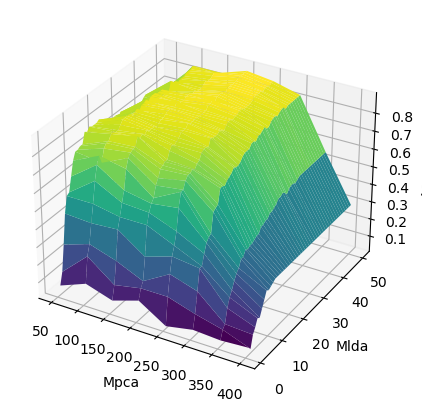
\includegraphics[width=0.8\linewidth]{image/mpca_mlda.png}

   \caption{Classification accuracy varying Mpca and Mlda}
   \label{fig:mpca_mlda}
\end{figure}

\begin{figure}[t]
  \centering
   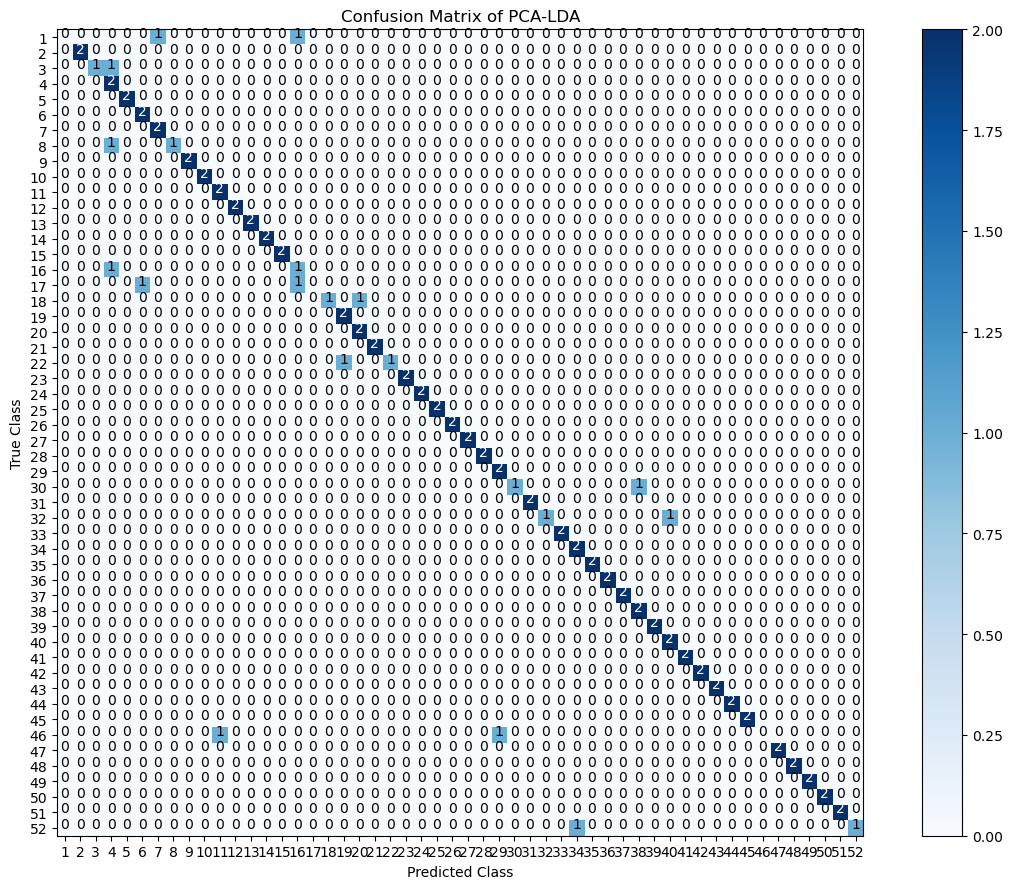
\includegraphics[width=0.8\linewidth]{image/q3_1_cm.png} % Seems better to move to Appendix,,

   \caption{Classification accuracy varying Mpca and Mlda}
   \label{fig:q3_1_cm}
\end{figure}

%-------------------------------------------------------------------------
\subsection{Result of PCA-LDA}

\cref{fig:q3_1_cm} is the confusion matrix of PCA-LDA classification result. As most of prediction result is on the diagonal entry, it indicates that most of prediction is successful. We take a closer look at success and failure cases. \cref{fig:q3_success} shows successfully predicted cases. Despite the different angles of the faces, the model infer the class accurately. \cref{fig:q3_fail} is failure cases. It seems that the prediction failed because of the similar glasses and face expression.

\begin{figure}[t]
  \centering
   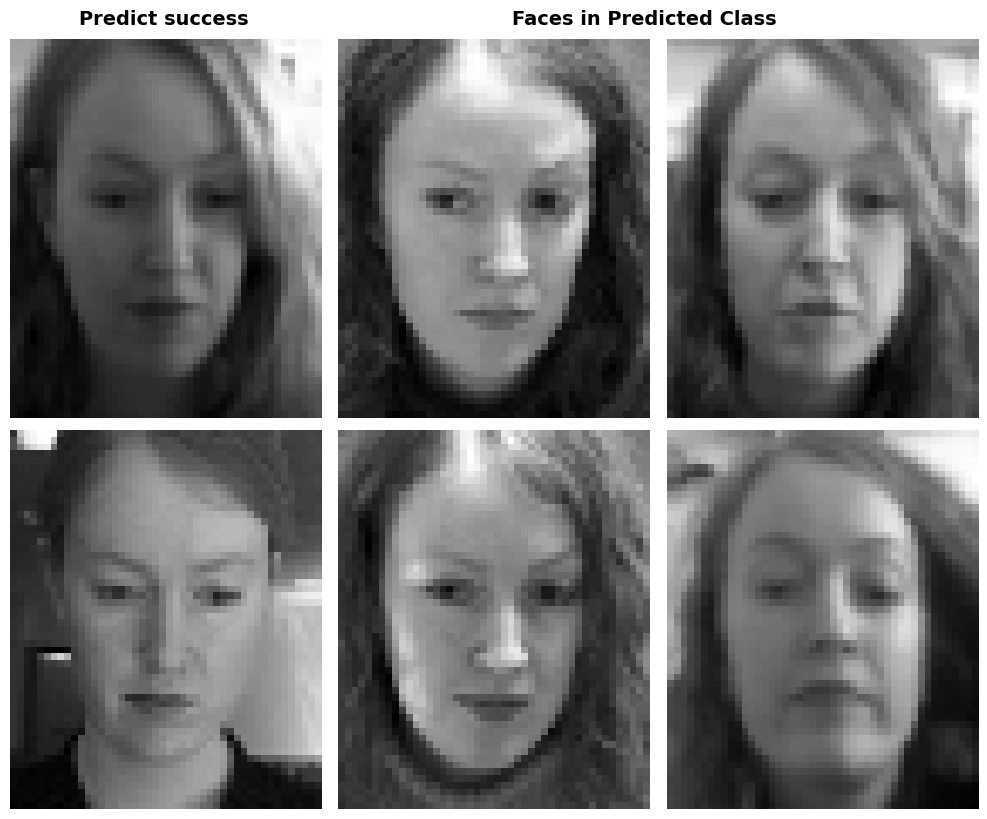
\includegraphics[width=0.8\linewidth]{image/q3_success.png}

   \caption{Classification accuracy varying Mpca and Mlda}
   \label{fig:q3_success}
\end{figure}

\begin{figure}[t]
  \centering
   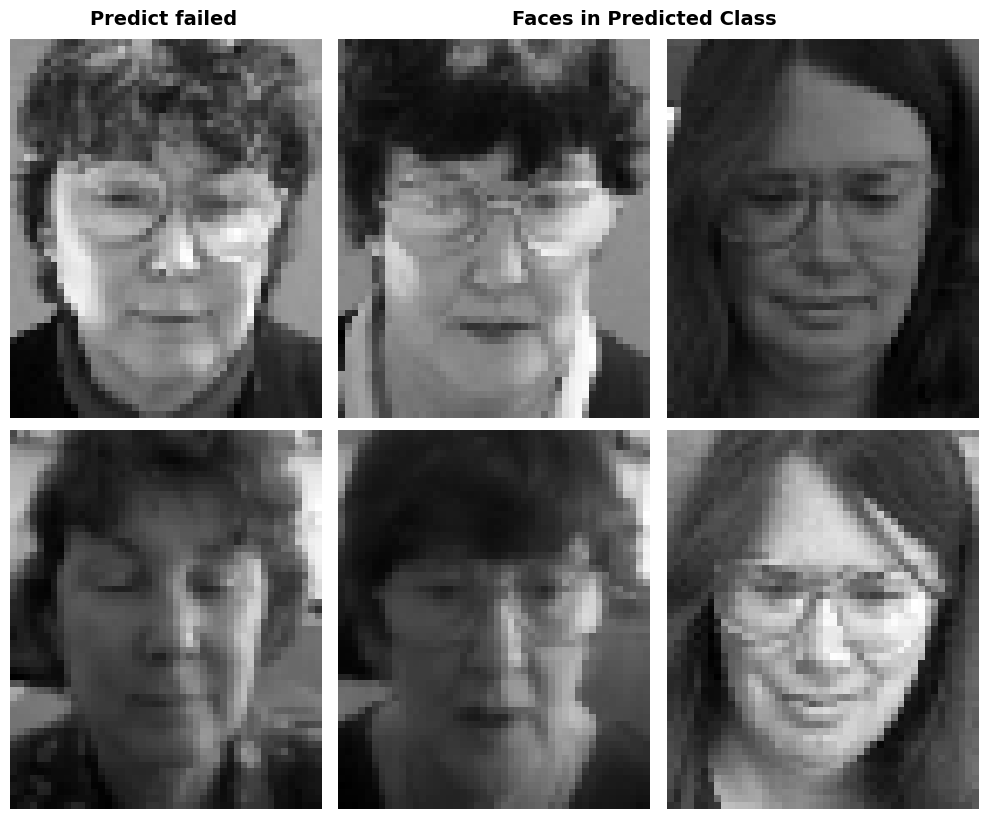
\includegraphics[width=0.8\linewidth]{image/q3_fail.png}

   \caption{Classification accuracy varying Mpca and Mlda}
   \label{fig:q3_fail}
\end{figure}

%-------------------------------------------------------------------------
\subsection{Time and Memory}
Comparison btw pca/pca-lda (accuracy), lda/pca-lda(time), pca/lda/pca-lda(memory)

%-------------------------------------------------------------------------
\subsection{PCA-LDA Ensemble}
For PCA-LDA Ensemble model, we combined two different types of models. The first type is randomization in feature space, which select vectors for pca projection randomly by a certain percentage. The second type is randomization in data sampling, which randomly subsampling the train data by a certain percentage. Both models were used in equal numbers. For combining prediction results of each models, we used 'majority voting' among various fusion rules. This is because, since our task is predicting class for classification and each classes don't have special meaning in numeric value, majority voting looks the most reasonable compared to other methods like averaging and finding maximum. 

%-------------------------------------------------------------------------
\subsection{Randomization}
randomization in feature space (m0)
randomization in data samples (subset\_rate)
randomization in model number (model\_num)
randomness parameter

%-------------------------------------------------------------------------
\subsection{Result of PCA-LDA Ensemble}
error (committee machine, individual models)
accuracy, confusion matrix
